\section{日本が狙うサイエンス}\label{cosmology.s3}

この章では、SKA計画で注目される宇宙論研究について我が国で進展が期待される科学的な課題について
以下にまとめる。

\ref{cosmology.s1.ss1}節で述べたように、現在我々が直面する宇宙論の重要な未解決問題は大きく
次の3つである:「インフレーションがどのように起こったのか」、「暗黒エネルギーの正体とは何か」、
「暗黒物質の正体は何か」である。
SKAのような低周波電波干渉計により、$30,000$平方度にわたる広範な天球を掃くだけでなく、
$z\gtrsim 5$のような高赤方偏移宇宙にまで到達可能であることから、
SKAの観測データを用いることでこれまでにない精度・規模の宇宙論観測が可能になる。

しかしその一方で、上記のような問題にアプローチしうるような精密宇宙論探査を
観測データから行うことは容易なことではない。
近傍宇宙では密度揺らぎは十分成長しており、
小スケールにおいて非線形性を無視することができなくなる。
非線形発展する系において精密な理論予言を行うことは非常に困難である。
近年多くの高精度$N$体計算や解析模型が提唱されているが、
常にモデルの自由度を内在することになってしまう。
さらに、小スケールではバリオンの物理を含む宇宙物理的な過程が介在することから
精密な予言を行うことを難しくしている。
これらの問題を打破し、そして宇宙論の未解決問題に決定打を与えるため、
SKA-JP宇宙論班では以下の3つを大きな活動の柱とする。
\begin{itemize}
\item[] (i) 超地平線スケール宇宙論によるインフレーション・暗黒エネルギーの探求
\item[] (ii) $21$cm線サーベイを用いた暗黒宇宙探査
\item[] (iii) 精緻な理論模型構築と暗黒エネルギー
\end{itemize}
それぞれは有機的に密接に関連しており、関係は相補的である。
以下、それぞれについて、研究の現状および問題点、研究計画を列挙する。\\

\begin{enumerate}
\item[{\bf (i)}] {\bf 超地平線スケール宇宙論}

上述の問題を打破する一つの方法は、地平線スケールを超えるような大スケールを探査することである。
超地平線スケールでは、密度揺らぎが線形領域に留まるだけでなく、
主たる宇宙物理的過程も介在しないことから非常にクリーンな理論予言が可能となる。
このとき、最大の障害となるのは宇宙の単一性により独立なモードを十分に取得することができず、
有限のサンプル数によるノイズ:コズミックバリアンス(Cosmic Variance; CV)を生む。
よって、SKAのようなほぼ全体を覆う広範な観測領域を持つ場合、CVを適切に取り扱うことが不可欠である。
我々宇宙論班は、コズミックバリアンスを取り扱う最も有望な手法として、
マルチトレーサー法~\citep{Seljak:2008xr}を積極的に取り入れることで、
観測データから宇宙論における有用な情報を効率的に抜き出すことを計画している。
この手法では、一つの観測データを少なくとも二つ以上の異なるバイアス因子を持つような
グループに分割することが本質的である。
複数のグループの相互相関を計算することで、バイアスの比の決定精度をショットノイズだけに
依存するようにすることができる。
これにより実効的にCVに依らずに観測量を制限することができる。
この手法の大きな利点としては、バイアスに依存する観測量であれば、観測量の如何に依存せずその効果を発揮する点である。
そのため、一つの手法で様々な宇宙論的諸問題に迫っていくことができる。

\begin{description}
\item {\bf 原始非ガウス性}

%宇宙最初期の指数関数的膨張期、いわゆるインフレーションがどのように起こったのかは現在においてもなお
%明らかになっておらず、宇宙論分野における最も重要な研究テーマの一つである。
インフレーションを決定付ける最後のピースは
%近年注目されているのは、宇宙大規模構造の種、つまり
インフレーションが導く原始揺らぎの統計性の検定である。
最もシンプルなインフレーション模型が
ほとんどガウス統計に従う揺らぎを生成することは以前より知られていた。
しかし、高エネルギー物理の理解が深まるにつれ、ガウス統計から大きく逸脱した揺らぎを生成するような模型の
存在が認知されている。
原始非ガウス性は模型に固有の理論予言を与えることから、あまた存在するインフレーション模型の選別に用いることができる。
この理論的研究は宇宙論班に在籍する研究者を含む多くの日本人が重要な寄与をしてきたという
実績があり、観測への応用においてもその素地を生かすことで大きな貢献が見込める。

既に\ref{cosmology.s1.ss1}節で議論したように、\eqref{eq:fNL def}式のように特徴づけるのが一般的である。
既に非線形パラメータ$f_{\rm NL}$に対して様々な観測から制限が与えられているが、
%既にPlanck衛星によるCMBの観測により、$f_{\rm NL}=2.7\pm 5.8$ ($68\%$ C.L.)という制限値が与えられている。
最もシンプルなインフレーション模型は$f_{\rm NL}={\cal O}(0.01)$という非常に小さい値を予言することから、
誤差を${\cal O}(0.01)$に抑えることが今後の宇宙論研究において重要な地位を占めることになる。
原始非ガウス性が存在する場合には、%銀河数密度揺らぎの背景にある暗黒物質揺らぎに対する
バイアスがスケールおよび赤方偏移依存性を持つことが近年指摘されており (\eqref{eq:scale dependent bias}式)、
銀河サーベイを用いてバイアスのスケール依存性を精密に測定することで原始非ガウス性を観測することができる。
CMBを用いた場合、将来観測であっても$\sigma (f_{\rm NL})={\cal O}(1)$までにしか到達できないのに対し、
SKAではこの観測の壁を越えてインフレーション模型に迫っていける可能性がある。

宇宙論班の山内、大栗、高橋によって、マルチトレーサー法をSKA連続波サーベイに応用することにより、
原始非ガウス性を探査する研究を既に実施し、論文としてまとめている~\citep{Yamauchi:2014ioa}。
実際的な観測に含まれる系統誤差を考慮に入れた場合であっても、マルチトレーサー法により
決定誤差を大きく抑制できることを明らかにし(図~\ref{fig:sigma_fNL_multitracer}左図)、
SKA連続波サーベイにより、CMBよりも強い制限$\sigma (f_{\rm NL})\lesssim 1$を得ることができることを示した。
さらに、光赤外観測計画Euclidとの結合解析により、$\sigma (f_{\rm NL})\approx 0.5$にまで到達しうることを
初めて示した実績がある (図~\ref{fig:sigma_fNL_multitracer}右図)。
この論文では、SKA連続波探査単体では銀河の赤方偏移については情報が得られないとして、最も悲観的な状況での
解析を行った。
しかし、%赤方偏移の情報の重要性についても議論しており、
光赤外観測との協働によりSKAで見出した銀河に赤方偏移情報を付与することで状況はさらに改善し、
$\sigma (f_{\rm NL})=0.01$を目指すことができる~\citep{Kitching:2015fra,Takahashi:2015zqa}。


%%%%%%%%%Figure%%%%%%%%%%%%%%%%%%%%%%%%%%%%%%%%%%%%%%%%%%%%%%%%%%%%%%%%%%%%%
\begin{figure}[t]
 \begin{minipage}{0.52\hsize}
 \begin{center}
%   \vspace{15pt}
   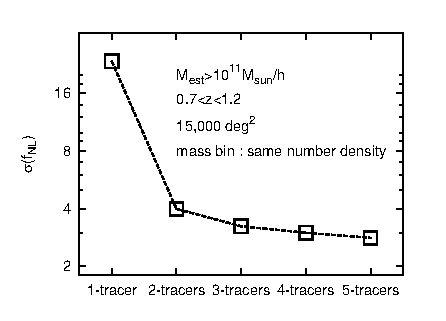
\includegraphics[width=1.0\linewidth]{cosmology/sigma_fNL_nTracer.eps} 
%   \vspace{10pt}
 \end{center}
 \end{minipage}
 \begin{minipage}{0.52\hsize}
 \begin{center}
   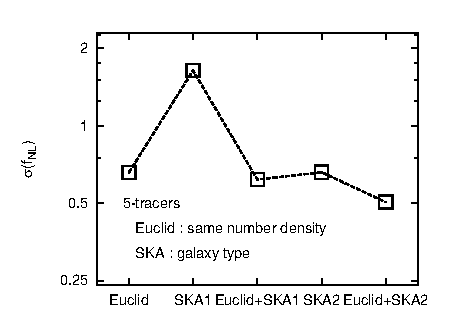
\includegraphics[width=1.0\linewidth]{cosmology/sigma_fNL_survey.eps} 
%  \vspace{-15pt}
 \end{center}
 \end{minipage}
\caption{(左図) トレーサーの分割数に対する非線形パラメータ$f_{\rm NL}$の決定精度。
%マルチトレーサー法を用いた結果、トレーサーを分割すればするほど実際にバイアスに含まれる
%原始非ガウス性の決定誤差が小さくなることを確認することができる。
(右図) サーベイ計画ごとの$f_{\rm NL}$の決定精度。
Euclidについては観測データから銀河質量を推定できるため、自由にトレーサーを分割できるとしているが、
SKAは銀河の形状タイプごとに分割し、それぞれに質量の推定値を付与することでバイアスを与えている。
\label{fig:sigma_fNL_multitracer}}
\end{figure}
%%%%%%%%%%%%%%%%%%%%%%%%%%%%%%%%%%%%%%%%%%%%%%%%%%%%%%%%%%%%%%%%%%%%%%%%%%%%
%<><><><><><><><><><><><><><><><><><><><><><><><><><><><><><><><><><><><><><><><><><><><><><><><><><>%
\begin{figure*}
\begin{center}
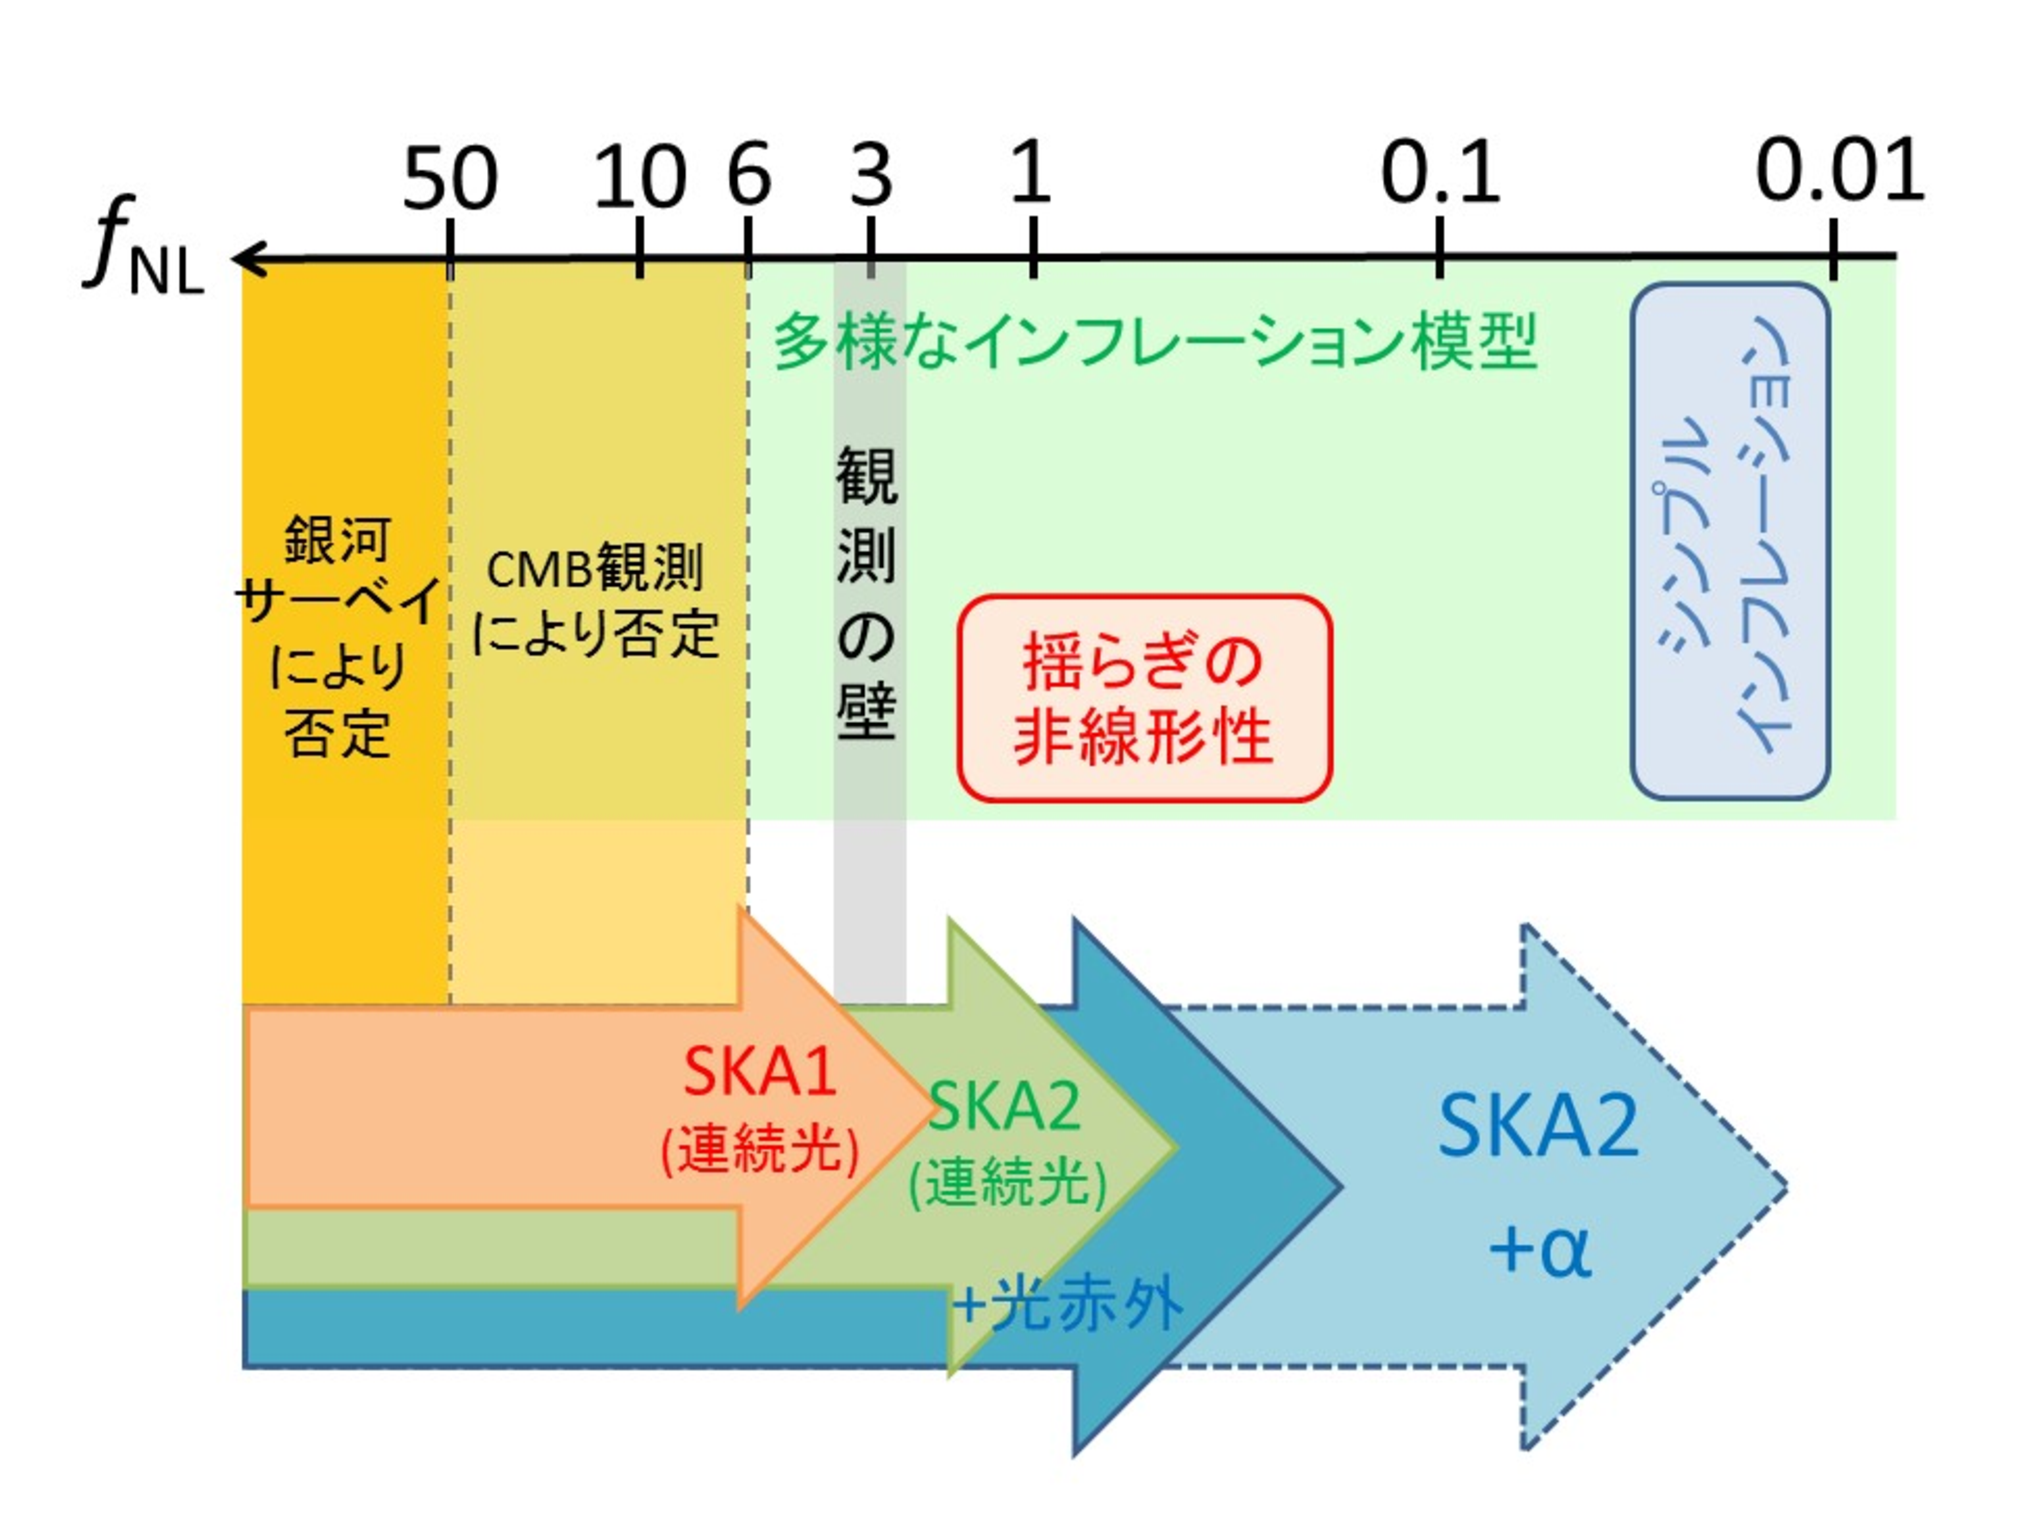
\includegraphics[width=100mm,clip]{cosmology/sigma_fNL_future.eps}
\caption{
SKAを用いた原始非ガウス性の探査における将来展望。
}
\label{fig:sigma_fNL_future}
\end{center}
\end{figure*}
%<><><><><><><><><><><><><><><><><><><><><><><><><><><><><><><><><><><><><><><><><><><><><><><><><><>%

この結果を踏まえ、SKA-JP宇宙論班として、
マルチトレーサー法を用いた原始非ガウス性の探査を行う。
以下より具体的な研究計画を以下に示す。

まず第一に我々は、より広いクラスの非線形パラメータに着目する。
原始非ガウス性は多点相関関数の形状に依存するため、上述したパラメータ$f_{\rm NL}$以外にも
多数のパラメータが存在することが知られている。
これらを網羅的に調べなければ、原始非ガウス性の全貌を明らかにすることはできない。
$f_{\rm NL}$以外の原始非ガウス性を探査する重要な点として、無矛盾条件の存在が挙げられる。
原始揺らぎが単一の場によって生成されるインフレーション模型を考えた場合、$f_{\rm NL}$と$4$点関数を特徴付ける
非線形パラメータ$\tau_{\rm NL}$の間に以下の関係が成立することが知られている~\citep{Boubekeur:2005fj,Okamoto:2002ik}:
\begin{align}
	\tau_{\rm NL}=\frac{36}{25}\left( f_{\rm NL}\right)^2
	\,.\label{eq:condition}
\end{align}
この無矛盾条件の可否を調べるためには、高次効果を適切に観測データから読み取る必要がある。
それは容易なことではないが、得られる情報は多岐にわたる。
無矛盾条件の破れを観測から見出した場合にはインフレーション模型に対する重要な示唆を与える。
特に、破れの原因として、インフレーションが複数の場によって引き起こされた可能性が盛んに議論されている。
最も単純なインフレーション模型は、質量の軽い単一のスカラー場により引き起こされるものであるが、
高エネルギー物理の観点に立った場合、宇宙初期に軽質量スカラー場がただの一つしかないことは不自然であり、
一般的には複数場が同時に揺らぎに寄与しうる(例えば\cite{Lyth:2001nq,Moroi:2001ct,Enqvist:2001zp})。
その際には上記の無矛盾条件は破れ、不等式$\tau_{\rm NL}\geq (36/25)(f_{\rm NL})^2$に一般化される
ことが指摘されている(須山-山口不等式~\cite{Suyama:2007bg})。
また、$\tau_{\rm NL}$以外にも複数のパラメータが存在し、それらを組み合わせることで模型間の
縮退すらもとくことができるようになる。
これらを探査することは、エネルギー的に宇宙を支配していない微小な成分の振る舞いを調べることに対応しており、
これまで知られていなかった初期宇宙を詳細に知ることが出来る。

様々なタイプの原始非ガウス性を探ることでインフレーション模型の選別において少なくない寄与をすることができるが、
SKAの文脈において$f_{\rm NL}$以外の非ガウス性の探査の研究はほとんど存在しない。
我々はここに着目し、SKAのような高精度観測を用いることで、様々なタイプの原始非ガウス性をスケールに依存するバイアスから
制限することを目指す。
また、原始非ガウス性パラメータの多くはバイアスに対してどのように依存するかはよく知られていない。
我々宇宙論班はこれまでの理論的研究によって培われた非ガウス性の知識を用いることでより広いクラスの原始非ガウス性が導く
バイアスを網羅的に探査していくことも行う。
これにより、初期宇宙、とりわけ「インフレーションがどのように起こったのか」という宇宙論の最も基本的な質問の一つに迫っていく。
\\


\item {\bf 暗黒エネルギーの探査}

宇宙を加速させている構成要素、いわゆる暗黒エネルギーの原因については
様々な提案がなされているが、研究者の間での統一された理解は存在しない。
%そのため、宇宙項以外の暗黒エネルギーとして理論的な要素の探求が様々な観点から行われている。
物質に新しいエネルギー源を導入することを諦め、重力を記述する理論を一般相対論から変更することで
実効的に暗黒エネルギーとして振る舞い得るようにすることが検討されている(修正重力理論)。
多くの修正重力理論の理論的な研究に対して、
我が国は多大な貢献をしているおり、深い理解に基づく洞察を観測に生かすことで大きな効果が得られると期待している。
これらの多くは標準的な宇宙論を超えるような高エネルギー物理から推測される効果を定性的に取り入れたものになっており、
観測的に探査することで例えば量子重力のような高エネルギー物理に対して示唆を与えることができる。

SKAによる高赤方偏移にわたる高精度により、暗黒エネルギーの時間変化を特徴付けるパラメータ、
例えば状態方程式$w$の時間進化(\eqref{eq:DE EOS def}および\eqref{eq:DE EOS}式)の制限は
大きく改善するものと期待できる。
さらに、SKAでは一般相対論のテストを非常によい精度で実行できる。
修正重力理論は典型的に密度揺らぎの発展史を大きく修正し、観測から密度揺らぎの成長率
を精密に探査することにより重力理論に強い制限を与えることができると期待される。

さて、暗黒エネルギーの探査とマルチトレーサー法との関連および研究計画について以下に示す。
既に述べたように、揺らぎの成長率$f$は、ドップラーシフトに対応する赤方偏移方向歪みを
通じて背景にある暗黒物質の揺らぎに対して有効バイアスの一部として振舞う(\eqref{eq:Pobs}式)。
そこで、上述したマルチトレーサー法を用いて銀河密度揺らぎのバイアスを高精度で決定することで発展因子についても
コズミックバリアンスによることなく決定することができる。
我々宇宙論班は、これまでの理論研究を素地とし、マルチトレーサー法を用いることで
これまでにない精度での暗黒エネルギー探査を目指す。
修正重力理論の理論的な研究に通じている研究者らが実際の観測データから制限する本研究計画は、
非常にユニークで日本独自の方向性を打ち出すことができると期待している。
\\
%また、近年ではCMBの観測結果を発端として、修正重力理論が導くテンソルモード、つまり重力波について
%活発な議論が行われている。
%低赤方偏移時代における重力波の影響は通常十分小さいためこれまでその寄与は無視されてきたが、
%計画されているような精細観測においてはその限りではない。
%原始重力波の振る舞いについても一般相対論から予言されるものから大きく変更を受ける可能性があり、
%CMB観測および重力波直接観測との協働も視野に入れ、研究を行っていく。
%\\

\item {\bf トレーサーの分類方法の改善}

山内らの研究~\citep{Yamauchi:2014ioa}によって、マルチトレーサー法を用いる場合、そのトレーサーの分類の仕方によって
制限の強さは大きく変わることが指摘されている。
これは原始非ガウス性だけに限らず、マルチトレーサー法に一般的に含まれる不定性であると考えられる。
トレーサーの分類の際には、バイアスを決定付ける銀河質量をなんらかの方法で推定する必要がある。
SKAのような電波観測の場合、銀河の質量を観測量から推定することは困難である。
これまでの研究においては銀河を形状で分類分けし、それぞれの形状タイプに経験的に知られている推定質量を
付与することでバイアスとの関連付けを行っている。
しかし、この手法は、銀河一つ一つについて形状タイプを適切に決める必要があり、さらに
形状タイプと推定質量との対応関係の付け方に強く依存している。
これらは大きな系統誤差の原因になる可能性が高く、精度のよい探査を実行するためには
系統誤差の原因をできる限り取り除くことが必要になる。
我々宇宙論班は、質量推定の制度を上げるため、SKA-JP銀河班と協働することで銀河の分類法、特に形状と質量との
関連についての理解を推し進めることを計画している。
また、形状タイプからの質量推定だけでなく、質量の推定を正確に行えるような新たな観測量を模索していく。

\end{description}

\vspace{0.2in}

\item[(ii)] {\bf $21$cm線観測を用いた暗黒宇宙探査}

SKAでは中性水素ガスの(赤方偏移した)$21$cm線輝線の観測を広範な天球面に対して行うことを計画している。
銀河等の光源がなくても中性水素原子さえ存在すれば観測可能であることから、銀河探査で観測できる時代より
さらに高赤方偏移($z\gtrsim 6$)の宇宙の情報を得ることができる。
宇宙がどのように再電離したのかを調べられるだけでなく、再電離期以前の物質の密度揺らぎも
測定することが可能である。
そのため、CMB観測と同様に宇宙論パラメータに制限を与えることが出来る。
特に、$21$cm線観測はCMB観測とは違い、異なる周波数が異なる赤方偏移を探査することに対応することから
$21$cm線トモグラフィーを行うことができる。
これによりサンプル数をCMB観測に比べて格段に多く取ることができる。
また、様々な赤方偏移での物質密度揺らぎを探査することによって、その成長率を見積もることができる点も
興味深い。
高赤方偏移の宇宙においては、近傍宇宙に比べてはるかに小さいスケールまで線形揺らぎで取り扱うことができる。
これらの事実により、非常にクリーンな宇宙論探査を行うことができると期待される。

SKA-JP宇宙論班の郡、大山、関口、高橋らによって、SKAの$21$cm線観測による宇宙論パラメータの決定精度が
CMBの将来観測単独の場合に比べて非常によいことが指摘されている~\citep{Kohri:2013mxa}。
研究計画(i)で高次相関の制限を行ったのに対し、
本研究では原始曲率揺らぎの$2$点関数、つまりパワースペクトルを特徴づけるパラメータについて考察している。
これらは相補的であり、どちらもインフレーション模型を区別するために重要なツールである。
これまで行われた多くの研究は、原始曲率揺らぎパワースペクトルを特徴づける、冪指数($n_{\rm s}$)、
冪指数の波数依存性($\alpha_{\rm s}$)についてのみ着目していた。
しかし、これだけでは多様なインフレーション模型を区別するには不十分である。
そのためにはより高次項($\beta_{\rm s}$)を導入するのが必要であるが、
一般に非常に小さいことから観測は困難だろうと思われていた。
本研究において、SKAのような精密な電波観測を用いることで高次項に対してCMB観測単独と比較し、非常に
強い制限を与えることができることが示唆された(図~\ref{fig:CMB+21cm_v2})。

%<><><><><><><><><><><><><><><><><><><><><><><><><><><><><><><><><><><><><><><><><><><><><><><><><><>%
\begin{figure*}
\begin{center}
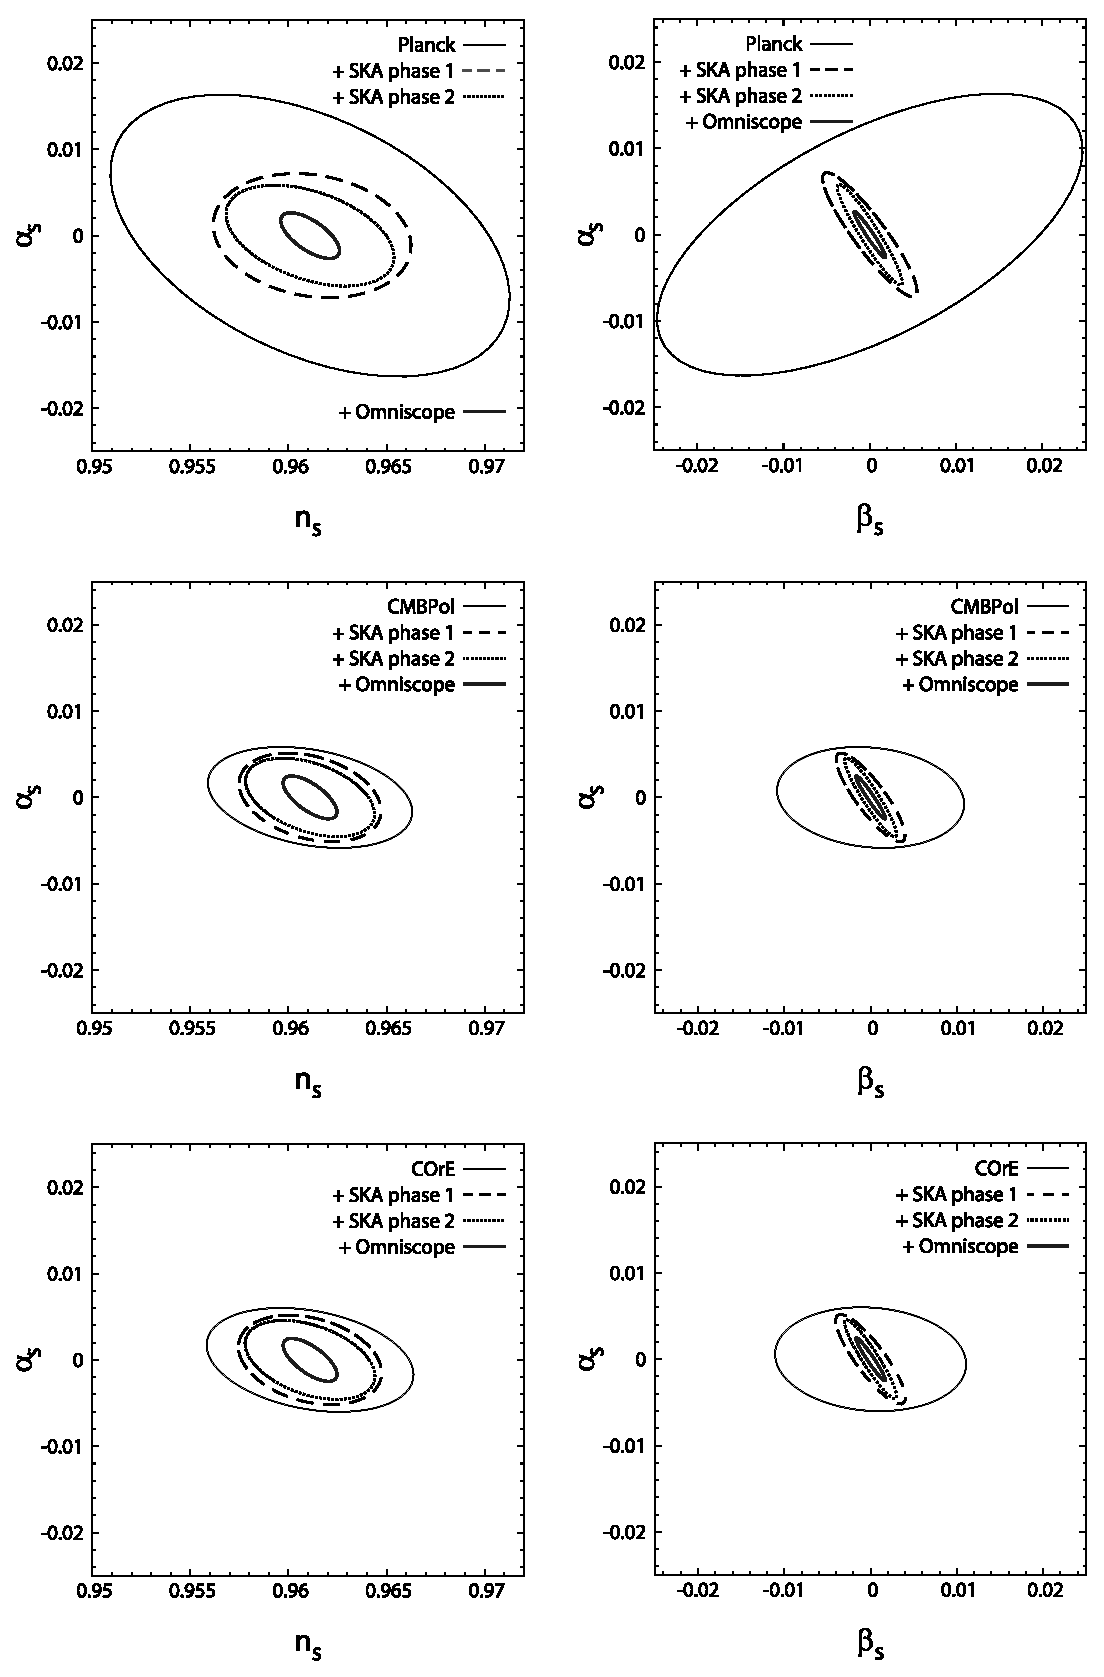
\includegraphics[width=120mm,clip]{cosmology/CMB+21cm_v2.eps}
\caption{
CMB観測 (Planck, CMBPol, COrE; \ref{cosmology.s1.ss2}節参照)およびSKA1/2による
結合解析を行った場合の$n_{\rm s}-\alpha_{\rm s}$および$\alpha_{\rm s}-\beta_{\rm s}$の
$95\%$C.L.決定精度。赤方偏移としては$6.8<z<10$を考慮。
CMB観測単独に比べて電波観測を考慮することにより非常に強い制限を与えることができる。
比較として、将来電波観測計画Omniscope~\citep{Tegmark:2009kv}による決定精度もプロットしている。
}
\label{fig:CMB+21cm_v2}
\end{center}
\end{figure*}
%<><><><><><><><><><><><><><><><><><><><><><><><><><><><><><><><><><><><><><><><><><><><><><><><><><>%

$21$cm線観測は原始曲率揺らぎパワースペクトルの探査だけではなく、素粒子物理に対するプローブとしても
用いることができる。
実際、郡、大山らによって$21$cm線観測によるニュートリノの性質に迫る研究が行われている~\citep{Oyama:2012tq}。
ニュートリノは電気的に中性でほとんど相互作用しない素粒子である。
素粒子標準模型ではニュートリノは質量がないとされてきたが、スーパーカミオカンデ実験が
ニュートリノ振動を発見したことを契機として、その後の研究の発展により、ニュートリノには大変小さいながら、
わずかに質量があることが明らかになってきている
(正確には質量差の存在が明らかになった)。
$3$世代のニュートリノには$3$種類の質量固有状態が混ざり合って存在していることは現在知られているが、
この質量固有状態のそれぞれの質量の値はわかっていない。
さらに、$3$つの質量のどれが軽く、どれが重いかという質量階層性についても理解されておらず、
ニュートリノ物理における大きな謎となっている。
ニュートリノはその小さい質量のため、密度揺らぎの発展を阻害する効果があるため、
宇宙観測から密度揺らぎの成長を精密に探査することでニュートリノの質量やその質量階層性、そして世代数について
明らかにできる可能性がある。
図~\ref{fig:hierarchy_ellipse_v3}に示すように、SKAではニュートリノの$3$つの質量の固有状態の
質量の和と世代数に対し、強い制限を与えることが出来、将来的には質量階層構造さえ決定できる
可能性があることを明らかにした。
また、同様にしてレプトン非対称性のような素粒子模型の詳細についても探査可能であることが示されている~\citep{Kohri:2014hea}。

本研究計画においては、SKAの$21$cm線観測を用いたこれまでにない高赤方偏移宇宙を
探査することで宇宙論パラメータの精密測定を目指す。
特に、素粒子物理をSKAのような電波探査を用いてプローブする研究は我が国が世界を牽引しており、
今後我々はこの研究をさらに発展させていく。
上述の研究において示されたように、$21$cm線観測を用いることで物質の微小な振る舞いの違いをも観測可能になる。
素粒子の諸性質はこれまで地上実験により確かめられてきた経緯があるが、その素粒子の性質を
SKAのような高精度宇宙観測によって明らかにすることができるという点でユニークな研究と言える。
また、研究計画(i)が超地平線スケールのバイアスされた密度揺らぎに着目しているのに対し、
(ii)では小スケールにおける物質密度そのものの振る舞いが主たる観測対象となっていることから、
研究計画(i)と(ii)は相補的な関係にある。
そこで、(i)で実施する予定の原始非ガウス性および暗黒エネルギーの検定について、(ii)においても
物質密度揺らぎの多点関数を観測することによる探査を行う。
さらに、我々は、SKAで行われる新しい観測手法であるHI強度マッピングサーベイ
(\ref{cosmology.s2.ss0}節)にも注目している。
これまで素粒子物理に動機付けられてこの手法を応用した研究はなく、大きな発展が期待できる。

$21$cm線による密度揺らぎの観測は、再電離期の物理に非常に鋭敏であるが、
再電離がどのように起こったかについてはいまだ理論的にも観測的にも解明されていない研究テーマである。
特に前景放射の除去は$21$cm線精密測定において最も重要な課題の一つである。
SKA-JP宇宙再電離班では、前景放射の除去を大きな柱としており、協働を目指したい。
特に、宇宙論班では模型の自由度の少ない精密な理論模型を構築していくことで、
一層の高精度化が達成できると期待している。
%また、異なる観測と組み合わせた解析についても検討していきたい。
%特に、CMB観測による重力レンズ効果を合わせることで、パラメータの縮退を解き、
%より強い制限が得られるだけでなく、異なる観測間で相互相関を取ることによって
%系統誤差を大きく抑制することができると期待している。

\vspace{0.2in}

%<><><><><><><><><><><><><><><><><><><><><><><><><><><><><><><><><><><><><><><><><><><><><><><><><><>%
\begin{figure*}
\begin{center}
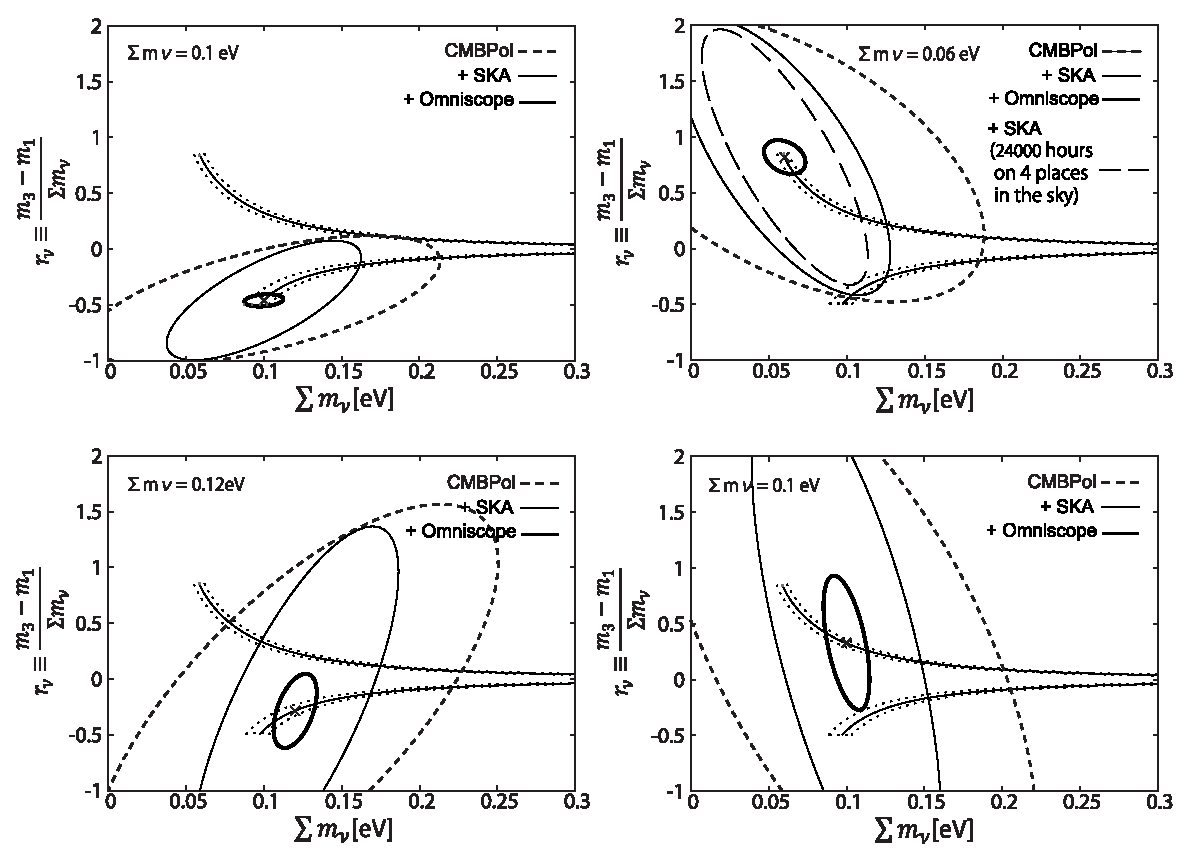
\includegraphics[width=110mm,clip]{cosmology/hierarchy_ellipse_v3.eps}
\caption{
各観測を用いた場合の$\sum m_\nu -r_\nu$の$90\%$C.L.決定精度。
赤方偏移としては$7.8<z<10.2$を考慮。
ここで、$r_\nu\equiv (m_3-m_1)/\sum m_\nu$である。
ニュートリノ振動実験によって許されている$r_\nu$の領域はそれぞれ
赤点線(正常階層)、青点線(逆階層)にはさまれている部分である。
それぞれの実線は$r_\nu$の基準の値を表している。
観測計画については図\ref{fig:CMB+21cm_v2}と同様。
SKAのような電波観測を考慮することにより、質量階層構造に対しても強い制限を与えることができる。
}
\label{fig:hierarchy_ellipse_v3}
\end{center}
\end{figure*}
%<><><><><><><><><><><><><><><><><><><><><><><><><><><><><><><><><><><><><><><><><><><><><><><><><><>%


\item[(iii)] {\bf 超地平線スケールでの精密な理論模型の構築と重力理論の検証}

赤方偏移方向歪みおよび重力レンズ効果による光度増幅効果については
小スケールにおいて重要となりえるため、これまでの観測においてもニュートン近似の補正項として
取り入れられてきた。
しかし、SKAで行われるほぼ全天を覆うような大スケールの観測ではもはやこれだけでは十分ではない。
観測者の視線上にある銀河数密度揺らぎや輝度温度揺らぎを観測するにあたり、背景時空そのものが揺らぎを受けて
一様等方時空からずれている効果を取り入れる必要がある。
その結果、観測体積が相対論的に変形する効果や曲がった時空上を光子が伝播してくることによる補正を
考慮することが必要になる。
%これらは観測対象の存在する局所的な重力ポテンシャルの情報のみならず、その時間変化にも影響している。
%相対論効果は小スケールでは安全に無視することができるが、超地平線スケールにおいては
%赤方偏移歪みや重力レンズ増幅効果と同程度の振幅を持ちえることが指摘されている。
これらの効果を考慮しない場合、大きくバイアスされた量を観測することになる。
よって、精密測定を行える観測においては、相対論効果まで含めた観測量を
考察することで初めて精緻な理論予言を与えることができる。

我々宇宙論班は、高精度理論予言を行うため、全ての効果を取り入れた詳細な理論模型構築を行う。
これらの効果はあらゆる観測量に対して寄与しうることから研究計画(ii)における$21$cm線観測に対しても
補正を考慮すべきである。
しかし、これまでにこれらを取り入れた研究についてはほとんど存在しないことから、
我が国が重要な寄与をできると期待している。
一方で、銀河サーベイの場合には、一般相対論効果も有効バイアスの一部として振舞うことから、
研究計画(i)で言及したマルチトレーサー法と非常に相性がよいと考えられる。
よって、有機的に相互の研究を関連付けて研究を推し進めて行くことで、よりよい理論予言を与えることができる。
さらに、重力理論が一般相対論と異なる場合には、
相対論的補正項の振る舞いも同様に変更を受けると推測される。
これにより予言値が大きくバイアスされる可能性があることから、我々は上述の研究計画によって得た知見を
踏まえることで、どの程度の補正が生じる可能性があるかを詳細に見積もることも行う。
この事実は、相対論的補正項を精密に探査することで、一般相対論のテストを行うことも可能であることを
示している。
研究計画(i)において成長率を用いて重力理論を検定することを行うが、本研究課題の結果を用いて
クロスチェックを行うことができることから相補的な関係があると言える。

\end{enumerate}
